
\begin{figure}[hbtp]
    \centering
    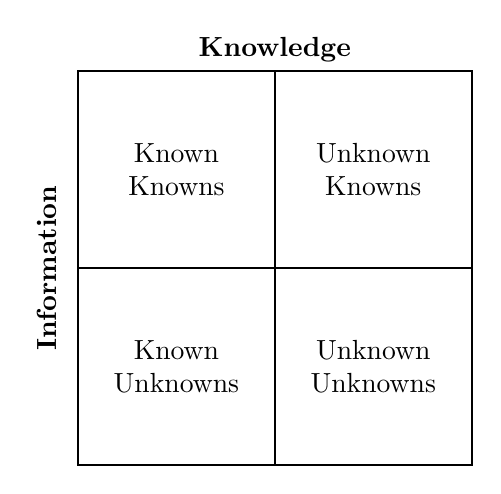
\begin{tikzpicture}[scale=1, every node/.style={align=center}]
        % Axes
        \draw[-, thick] (-2.5,0) -- (2.5,0);
        \node[rotate=90] at (-2.9, 0) {\textbf{Information}};
        \draw[-, thick] (0,-2.5) -- (0,2.5);
        \node[above] at (0, 2.5) {\textbf{Knowledge}};

        % Quadrants
        \draw[thick] (-2.5,-2.5) rectangle (2.5,2.5);

        % Labels
        \node at (-1.25,1.25) {Known\\ Knowns};
        \node at (-1.25,-1.25) {Known\\ Unknowns};
        \node at (1.25,1.25){Unknown\\ Knowns};
        \node at (1.25,-1.25){Unknown\\ Unknowns};

    \end{tikzpicture}
    \caption{Conceptual diagram, now called the Rumsfeld Matrix, can be used to describing the relationship between knowledge of a system and its properties.}
    \label{fig:rumsfeld}
\end{figure}
